\subsection{Hierarchical Clustering}
\begin{figure}
  \begin{minipage}[b]{0.5\columnwidth}
    \centering
    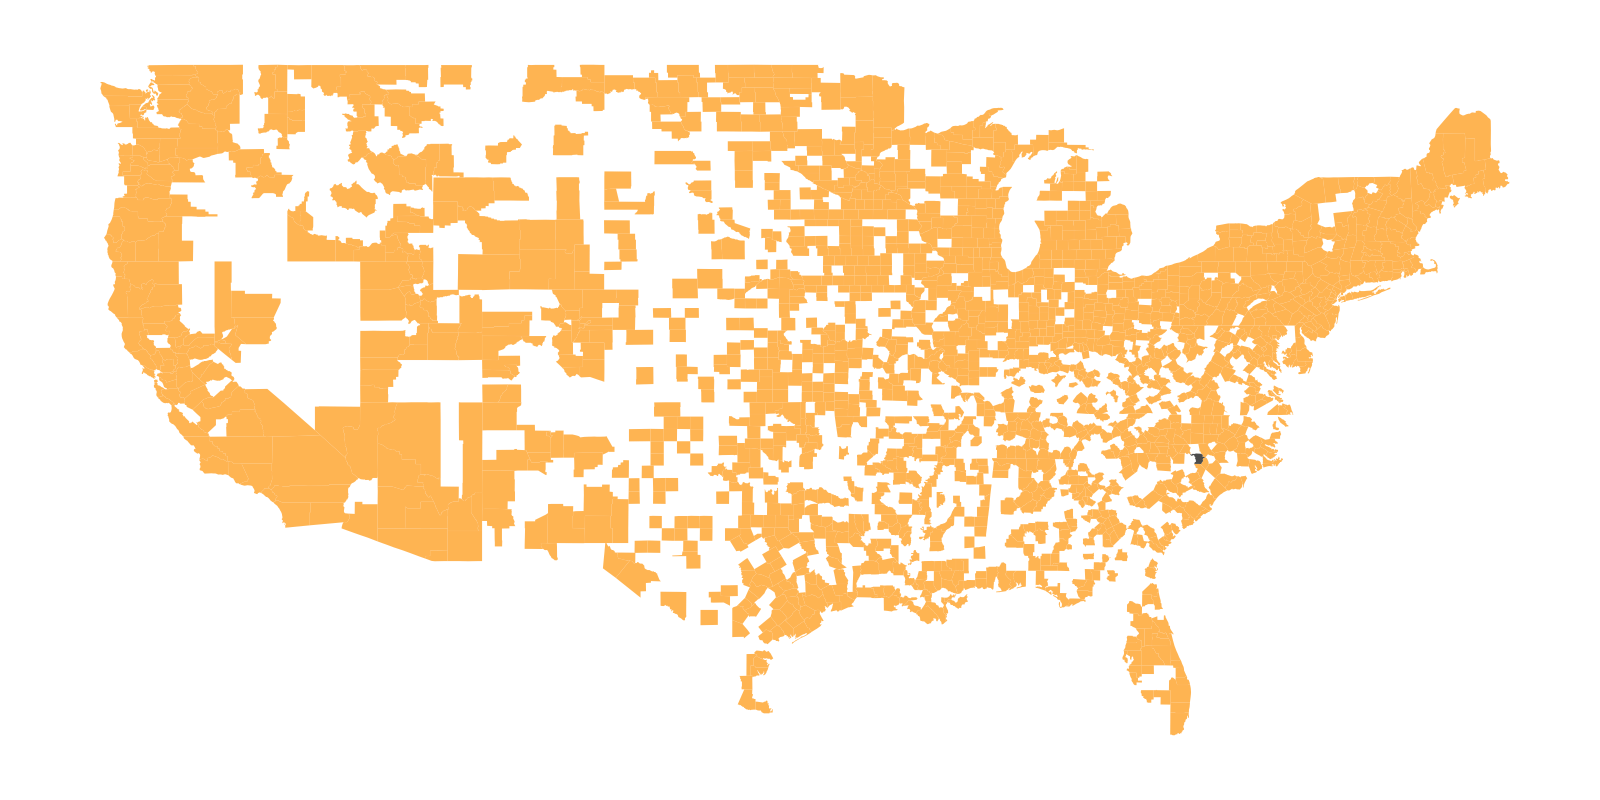
\includegraphics[width=\columnwidth]{fig/hierarchical1.png}
    \subcaption{Depth=1}\label{subfig:hierarchy1}   
  \end{minipage}
  \begin{minipage}[b]{0.5\columnwidth}
    \centering
    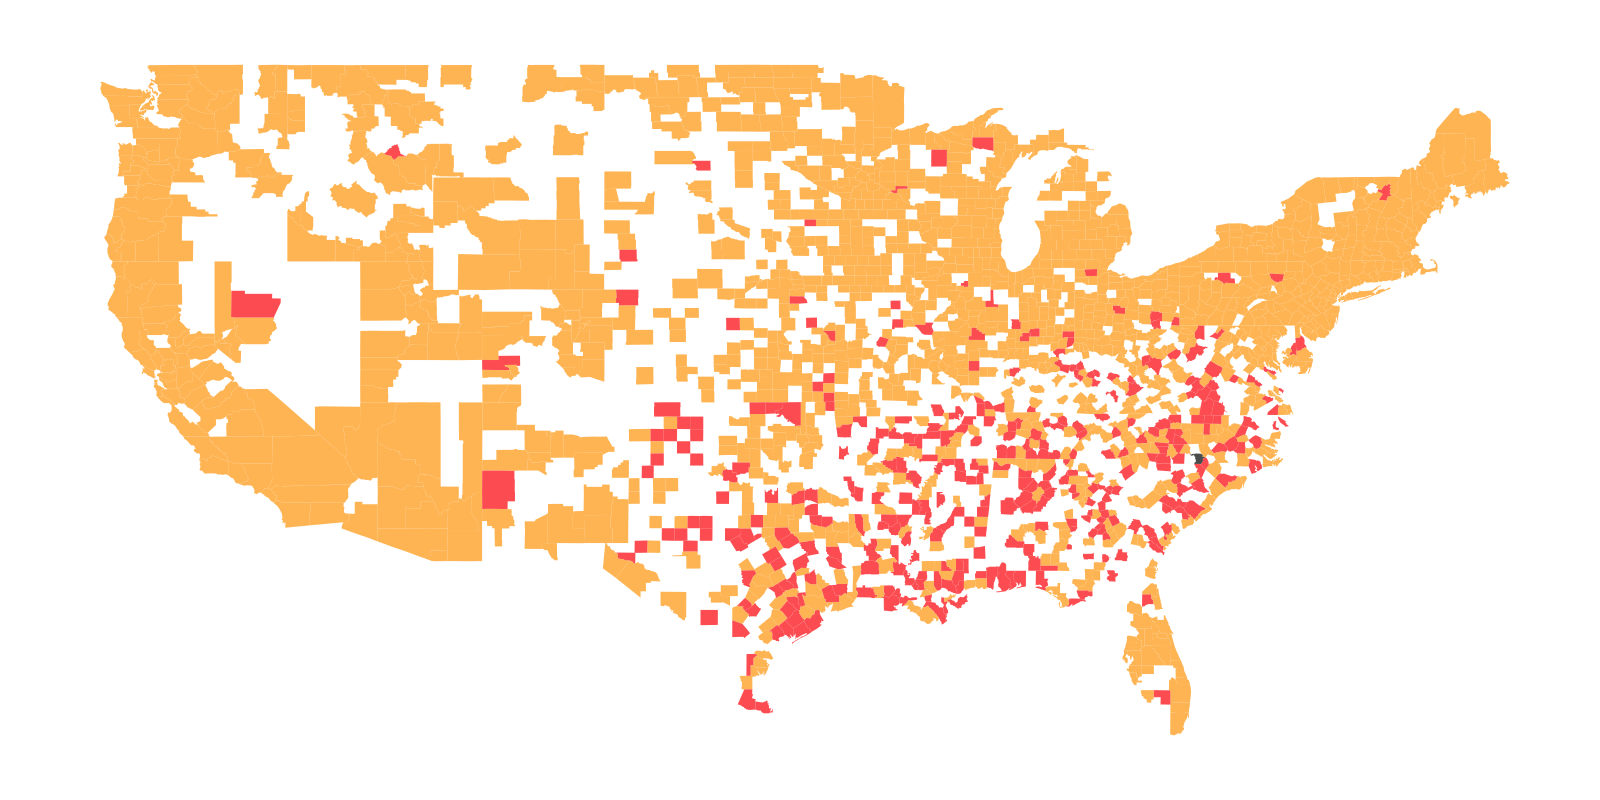
\includegraphics[width=\columnwidth]{fig/hierarchical2.png}
    \subcaption{Depth=2}\label{subfig:hierarchy2}
  \end{minipage}\\
  \begin{minipage}[b]{0.5\columnwidth}
    \centering
    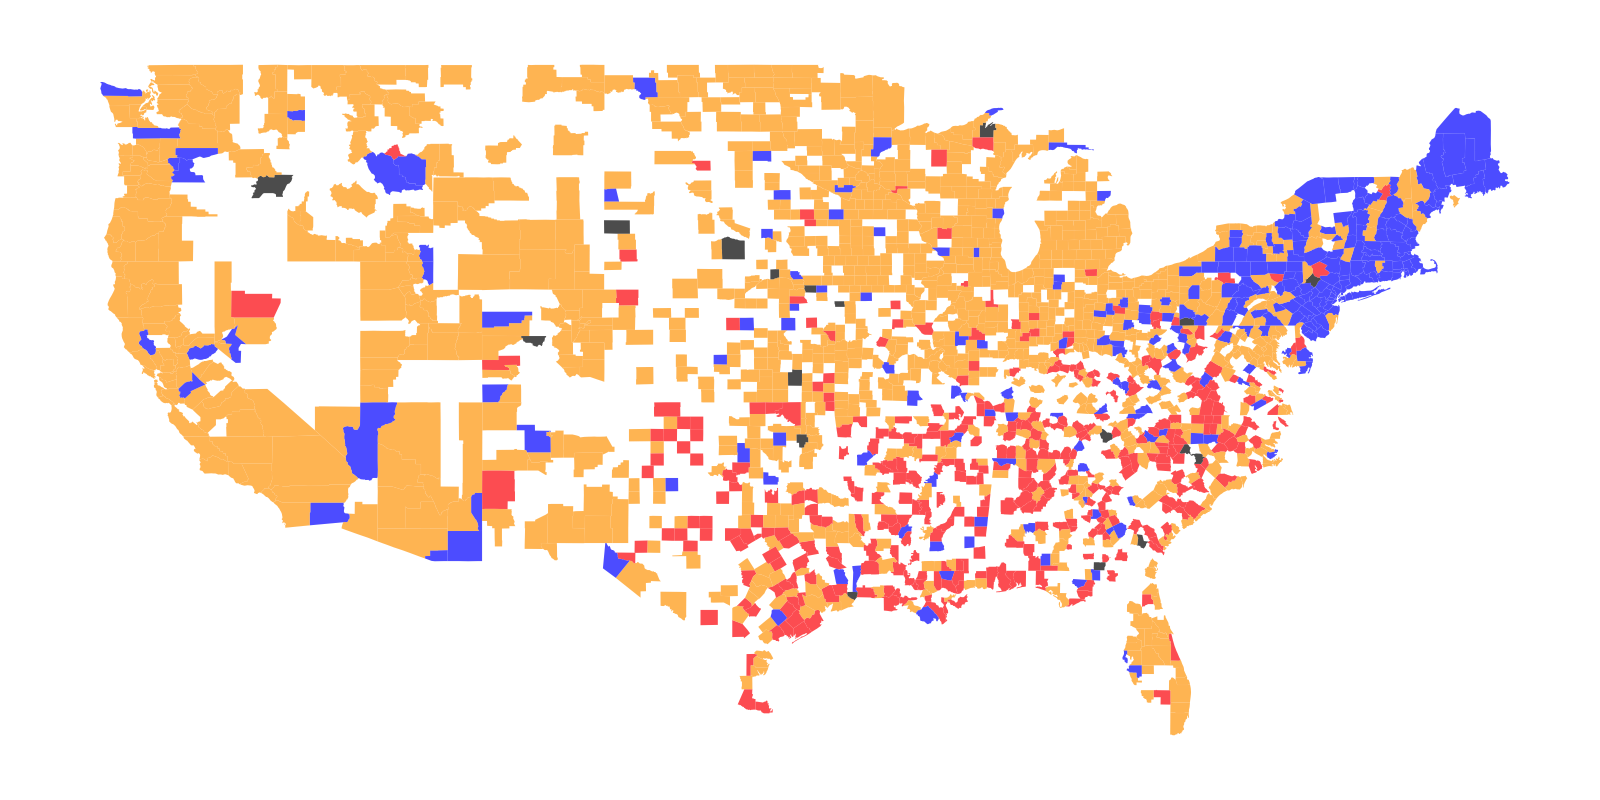
\includegraphics[width=\columnwidth]{fig/hierarchical3.png}
    \subcaption{Depth=3}\label{subfig:hierarchy3}
  \end{minipage}
  \begin{minipage}[b]{0.5\columnwidth}
    \centering
    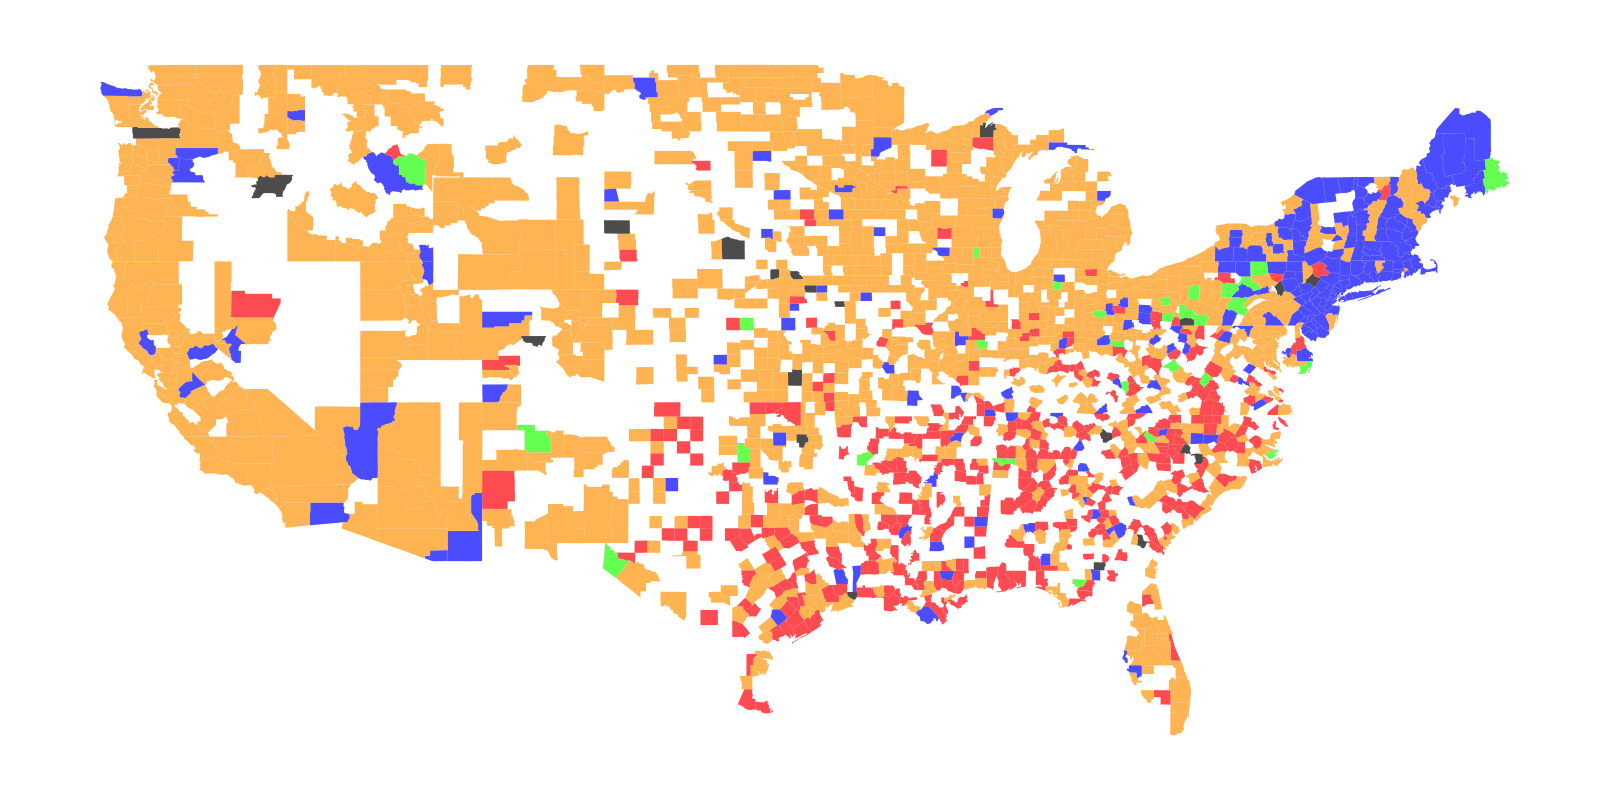
\includegraphics[width=\columnwidth]{fig/hierarchical4.png}
    \subcaption{Depth=4}\label{subfig:hierarchy4}
  \end{minipage}\\
  \begin{minipage}[b]{0.5\columnwidth}
    \centering
    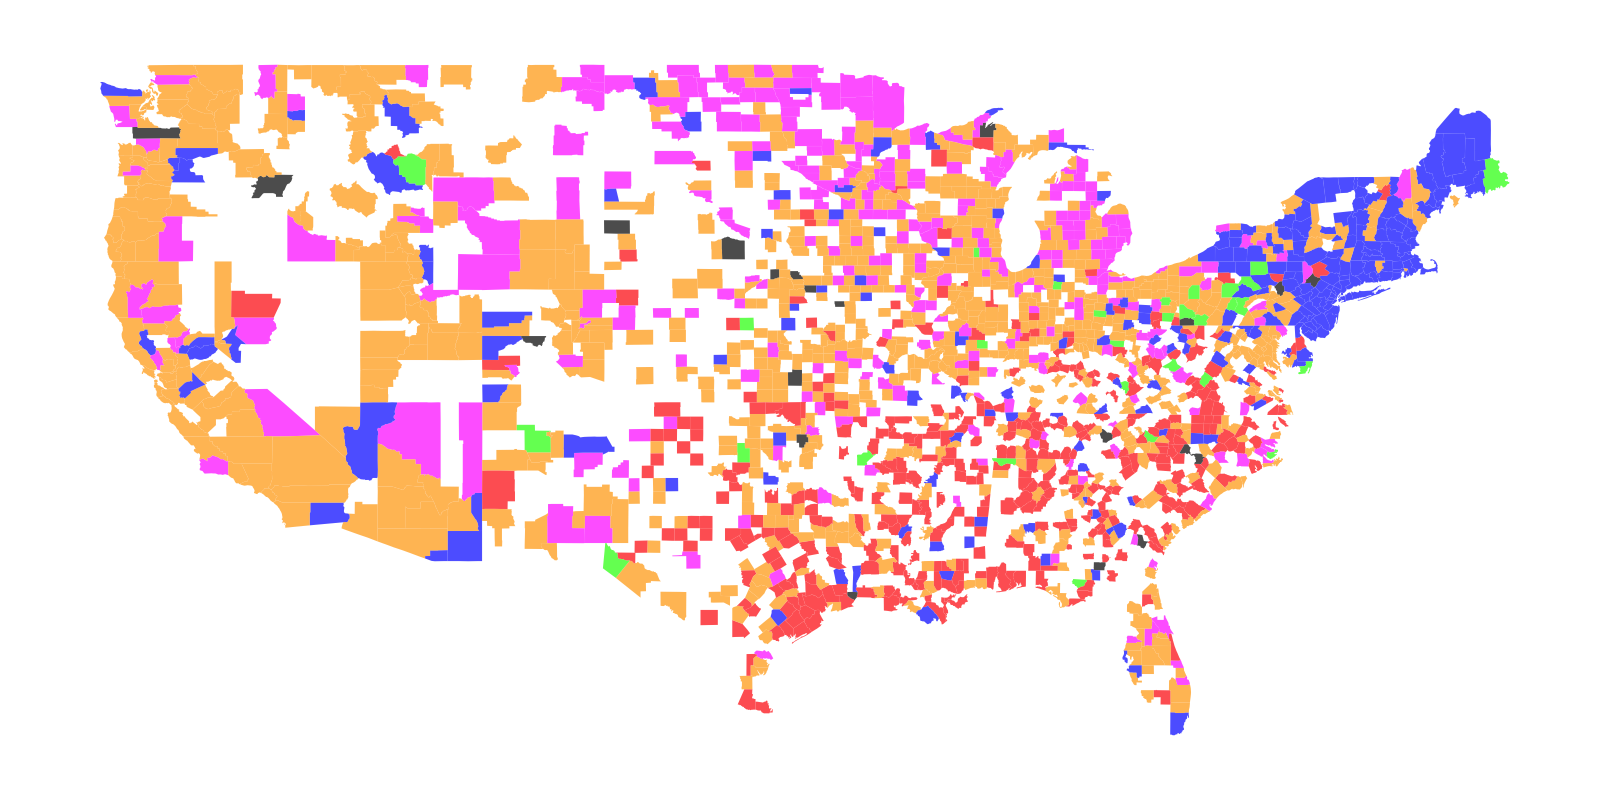
\includegraphics[width=\columnwidth]{fig/hierarchical5.png}
    \subcaption{Depth=5}\label{subfig:hierarchy5}
  \end{minipage}
  \begin{minipage}[b]{0.5\columnwidth}
    \centering
    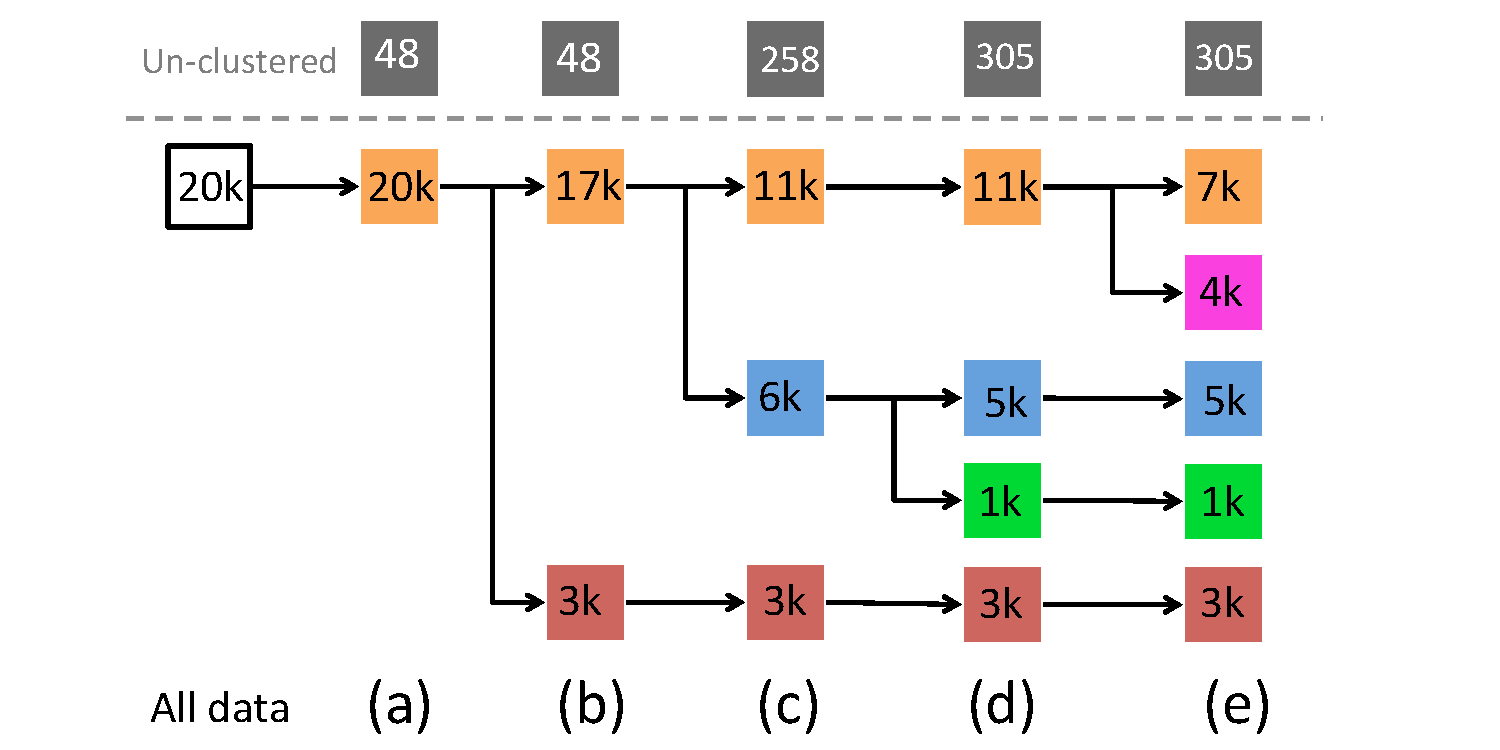
\includegraphics[width=\columnwidth,height=0.4\columnwidth]{fig/hierarchy.pdf}
    \subcaption{The hierarchy.}\label{subfig:hierarchy}
  \end{minipage}\\
  \caption{Hierarchical clustering. (a)-(e) gives clustering map at different hierarchy depth. (f) shows the hierarchy and number of observations that fall into each cluster.}
  \label{fig:hierarchy}
\end{figure}

\qquad  {\it Hierarchical clustering} is another method for clustering which finds a hierarchy of clusters. The result of hierarchical clustering can be presented as a dendrogram, a tree-like structure with a depth of $n-1$, where $n$ is the number of observations. At each depth, the dendrogram specifies which cluster can be further splitted into two small clusters, thus constructing the hierarchy. 

\qquad  By applying hierarchical clustering to our dialet dataset, we seek to find possible hierarchies in dialect regions. In other words, are there dialect regions that are closer to each other? Which dialect region has the most dissimilar language?

\qquad  When we apply hierarchical clustering to the datast, we find the following decisions to be relevant:

\begin{itemize}
\item \textbf{Sampling} We soon realize that we have to sample the dataset for faster processing. Hierarchical cluster requires pre-computing a pair-wise dissimilarity matrix between all observations. With 43265 observations, and 4 bytes per dissimilarity value in R, storing the matrix requires 6.97 GB of memory. This is beyond the memory capacity of any single machine we have. One way to reduce memory footprint is to trade off computation speed by creating dissimilarity values only when needed. For example, with {\it fastcluster::hclust.vector}, we don't need to create the matrix and finish one run of clustering with $\sim$67 minutes. We eventually decided to down-sample the data by half so that we could fit the entire dissimilarity matrix (1.6GB) in memory. This allows us to perform fast ($\sim$15s/run) clustering with various settings. We find that half sampling has limited impact on the findings we reach.

\item \textbf{Clustering Type} There are two types of hierarchical clustering: \textbf{Agglomerative} and \textbf{Divisive}, differentiated by how the computation starts. \textbf{Agglomerative} starts with each observation as a single cluster, and merge pairs of clusters until only one cluster is left. \textbf{Divisive} starts with a single cluster with all observations, and split clusters recursively until each observation has its own cluster. We choose \textbf{Agglomerative} due to lack of efficient \textbf{Divisive} implementations. 

\item \textbf{Dissimilarity Metric} determines how distance between two observations is calculated. We choose ``Manhattan distance'', which effectively captures how many questions a pair of participants have different answers (scaled by 2).

\item \textbf{Linkage Metric} determines how distance between two clusters are computed. We tried ``Single''(nearest neighbor method), ``Average'', ``Complete''(furthest neighbor method), ``Median'', ``Centroid'' and ``Ward''(minimizing within-cluster sum of squares). While most of the metrics lead to clusters of extreme size difference, we find ``Complete'' and ``Ward'' to be useful for generating clusters with similar diameters. 
\end{itemize}

\qquad  Figure~\ref{subfig:hierarchy} shows the hierarchy of first five depths when using the ``Complete'' metric. Each color box represents a cluster separated at that depth, with the number of samples in that cluster. Moving down the hierarchy, at each depth, one cluster is split into two small clusters at the next depth. This means that 1) the two small clusters are the closest pair at their depth; 2) the two small clusters are the furthest pair at one depth lower. 

\qquad  With the above observations, let's look at Figure~\ref{subfig:hierarchy1}$\sim$\ref{subfig:hierarchy5}, where we show the clusters on the geographic map. The first thing we notice is that the {\em Southern} dialect region is the first region to be identified, as shown in Figure~\ref{subfig:hierarchy2}. This means that the {\em Southern} region is most different compared to the rest of the country. With ``Ward'' as the linkage metric, the first identified region is the {\em New England East} region in northeast, which happens to be the second identified region under ``Complete'', as shown in Figure~\ref{subfig:hierarchy3}. Going downward the hierarchy, it is less clear that which specific region is identified, although clustering effect could still be observed. Compare the eventual separation in Figure~\ref{subfig:hierarchy5}, we find that clustering is noisier compared to k-means. We attribute this to the non-iterative nature (a observation will not be moved out of a cluster) of hierarchical clustering, as well as the fact that both linkage metrics we use, ``Complete'' and ``Ward'', are not robust to outliers.

\qquad  An animated version of the clustering results can be accessed at \url{https://goo.gl/photos/7udEt9JFmDVjw7676}.